% Copyright (c)  2024  sg4e.
% Permission is granted to copy, distribute and/or modify this document
% under the terms of the GNU Free Documentation License, Version 1.3
% with no Invariant Sections, no Front-Cover Texts, and no Back-Cover Texts.
% A copy of the license is included in the git repo.

\documentclass[aspectratio=169]{beamer}
\usepackage{graphicx}
\usepackage{tikz}
\usepackage{CJKutf8}

\newcommand{\idolcaption}[2]{
    \begin{minipage}{0.15\textwidth}
        \includegraphics[width=\linewidth]{#1}
        \vspace{0.2em}
        \centering
        \tiny{#2}
    \end{minipage}
}

\usetheme{Luebeck}

\title{hololive}
\subtitle{The most successful vtuber organization in the world}
\author{sg4e}
\date{November 2, 2024}
\institute{sp0cktober 2024}

\begin{document}
\maketitle

\begin{frame}{What is hololive?}
    \begin{itemize}
        \item hololive is a vtuber \textit{talent agency}
        \begin{itemize}
            \item Independent vtubers apply, audition, and interview to become \textit{members} of hololive
            \item If accepted, independent vtubers cease their previous activities and \textit{reincarnate} with a new virtual avatar and persona
            \item Avatars are commissioned from famous artists (Fate, Steins;Gate, Fire Emblem) and converted into models by experienced \textit{riggers}
        \end{itemize}
        \item hololive is a \textit{multimedia agency}
        \begin{itemize}
            \item hololive members publish original music, voice dramas, and sometimes even illustrations
            \item hololive coordinates large-scale concerts and performances of their members
        \end{itemize}
        \item hololive is wholly owned and operated by COVER Corporation
    \end{itemize}
    \begin{center}
        
\includegraphics[width=\linewidth,height=0.2\textheight,keepaspectratio]{images/hololive_logo.png}
    \end{center}
\end{frame}

\begin{frame}{What is COVER Corporation?}
    \begin{columns}
        \begin{column}{0.75\textwidth}
            \begin{itemize}
                \item Cover Corporation is the parent company of hololive
                \item Name derives from \underline{Co}mmunication + \underline{Vir}tual = COVER
                \item Classified as a technology and entertainment company
                \item Publicly traded on the Tokyo Stock Exchange as of 2023
                \item 973 million yen ($\approx$ \$6.3 million USD) as capital with 409 employees
                \item Managed and directed by CEO Tanigo Motoaki \begin{CJK}{UTF8}{min}谷郷元昭\end{CJK}
                \begin{itemize}
                    \item Also known by fans as YAGOO
                    \item Ranked as Japan's 3rd biggest entrepreneur by \textit{Forbes JAPAN} in 2023
                \end{itemize}
            \end{itemize}
        \end{column}
        \begin{column}{0.25\textwidth}
            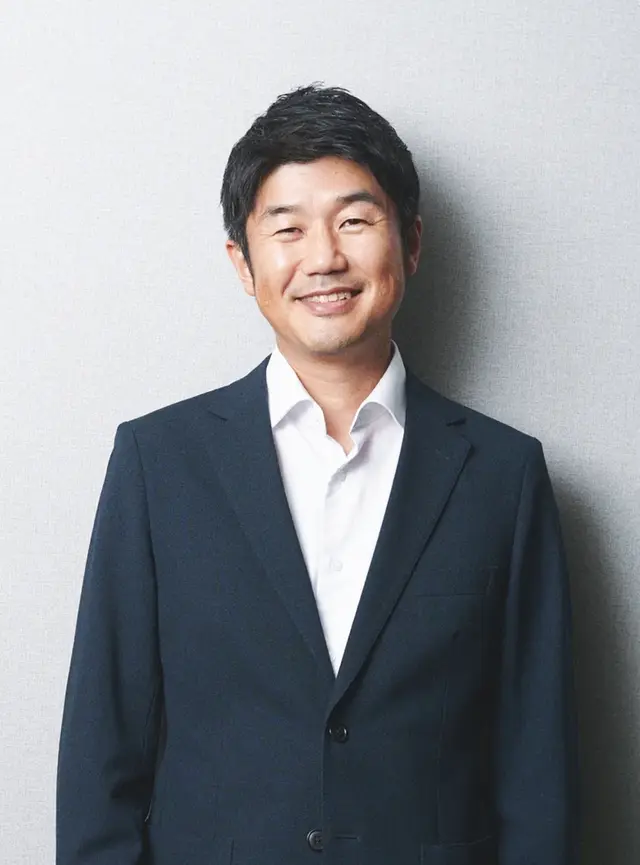
\includegraphics[width=\linewidth]{images/yagoo.png}
        \end{column}
    \end{columns}
\end{frame}

\begin{frame}{Humble Beginnings}
    \begin{itemize}
        \item First member debuted on September 7, 2017: Tokino Sora \begin{CJK}{UTF8}{min}ときのそら\end{CJK}, with the backstory of being a high-schooler with a dream of becoming an idol
        \item Robocosan \begin{CJK}{UTF8}{min}ロボ子さん\end{CJK} debuted on March 9, 2018, an ultra-high-tech robot
        \item Sakura Miko \begin{CJK}{UTF8}{min}さくらみこ\end{CJK} debuted on August 1, 2018, a shrine maiden
        \item Original designs were kept simple with themes that had general appeal; motion-capture tech was relatively primitive
        \item Future members would debut as groups, enumerated as \textit{generations} or \textit{gens}
    \end{itemize}
    \begin{minipage}{0.3\textwidth}
        \centering
        
\includegraphics[width=.3\linewidth]{images/sora.png}
    \end{minipage}
    \begin{minipage}{0.3\textwidth}
        \centering
        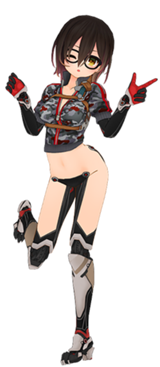
\includegraphics[width=.3\linewidth]{images/roboco.png}
    \end{minipage}
    \begin{minipage}{0.3\textwidth}
        \centering
        
\includegraphics[width=.3\linewidth]{images/miko.png}
    \end{minipage}
\end{frame}

\begin{frame}{Internal Composition}
    \centering
    \resizebox{\textwidth}{!}{ % Scales to frame width
        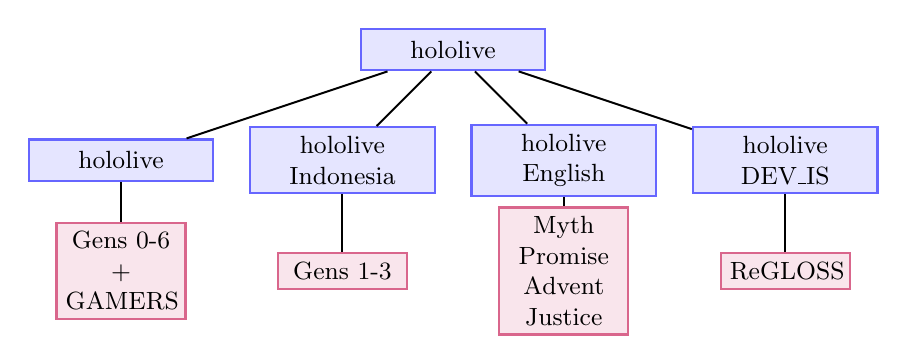
\begin{tikzpicture}[
            sibling distance=8em,
            level distance=4em,
            edge from parent/.style={draw, line width=.25mm},
            every node/.style={align=center, font=\small}
        ]
        
        % Define styles for nodes
        \tikzset{
            main/.style={rectangle, draw=blue!60, fill=blue!10, thick, minimum height=1.5em, text width=6em, align=center},
            subgroup/.style={rectangle, draw=purple!60, fill=purple!10, thick, minimum height=1em, text width=4em, align=center}
        }
        
        % Root node
        \node[main] (hololive) {hololive} 
            % Level 1: Branches
            child { node[main] (hololiveJapan) {hololive}
                % Level 2: Subgroups
                child { node[subgroup] {Gens 0-6\\+\\GAMERS} }
            }
            child { node[main] (hololiveID) {hololive Indonesia}
                child { node[subgroup] {Gens 1-3} }
            }
            child { node[main] (hololiveEN) {hololive English}
                child { node[subgroup] {Myth\\Promise\\Advent\\Justice} }
            }
            child { node[main] (devis) {hololive DEV\_IS}
                child { node[subgroup] {ReGLOSS} }
            };
        
        \end{tikzpicture}
    }
\end{frame}

\begin{frame}{Notable Members}
    \begin{itemize}
        \item Gawr Gura, the most subscribed vtuber (in the world!) (4.52M subs)
        \item Houshou Marine \begin{CJK}{UTF8}{min}宝鐘マリン\end{CJK}, the most subscribed active Japanese-language vtuber (3.52M subs)
        \item Kobo Kanaeru, the most subscribed Indonesian-language vtuber (2.59M subs)
        \item Hoshimachi Suisei \begin{CJK}{UTF8}{min}星街すいせい\end{CJK}, Gold certification from the Recording Industry Association of Japan for her 2024 single ``Bibbidiba" \begin{CJK}{UTF8}{min}ビビデバ\end{CJK} ($>$50 million plays on streaming platforms)
        \item Hakui Koyori \begin{CJK}{UTF8}{min}博衣こより\end{CJK}, 3rd most superchat revenue in 2023 (\$564k USD, 1st among non-religious channels)
    \end{itemize}
    \begin{center}
        \idolcaption{images/gura.png}{Gawr Gura}\hspace{0.01\textwidth}
        \idolcaption{images/marin.png}{Houshou Marine}\hspace{0.01\textwidth}
        \idolcaption{images/kobo.png}{Kobo Kanaeru}\hspace{0.01\textwidth}
        \idolcaption{images/suisex.png}{Hoshimachi Suisei}\hspace{0.01\textwidth}
        \idolcaption{images/koyori.png}{Hakui Koyori}
    \end{center}
\end{frame}

\begin{frame}{``Together, Let's Create Culture Loved by All''}
    \centering
    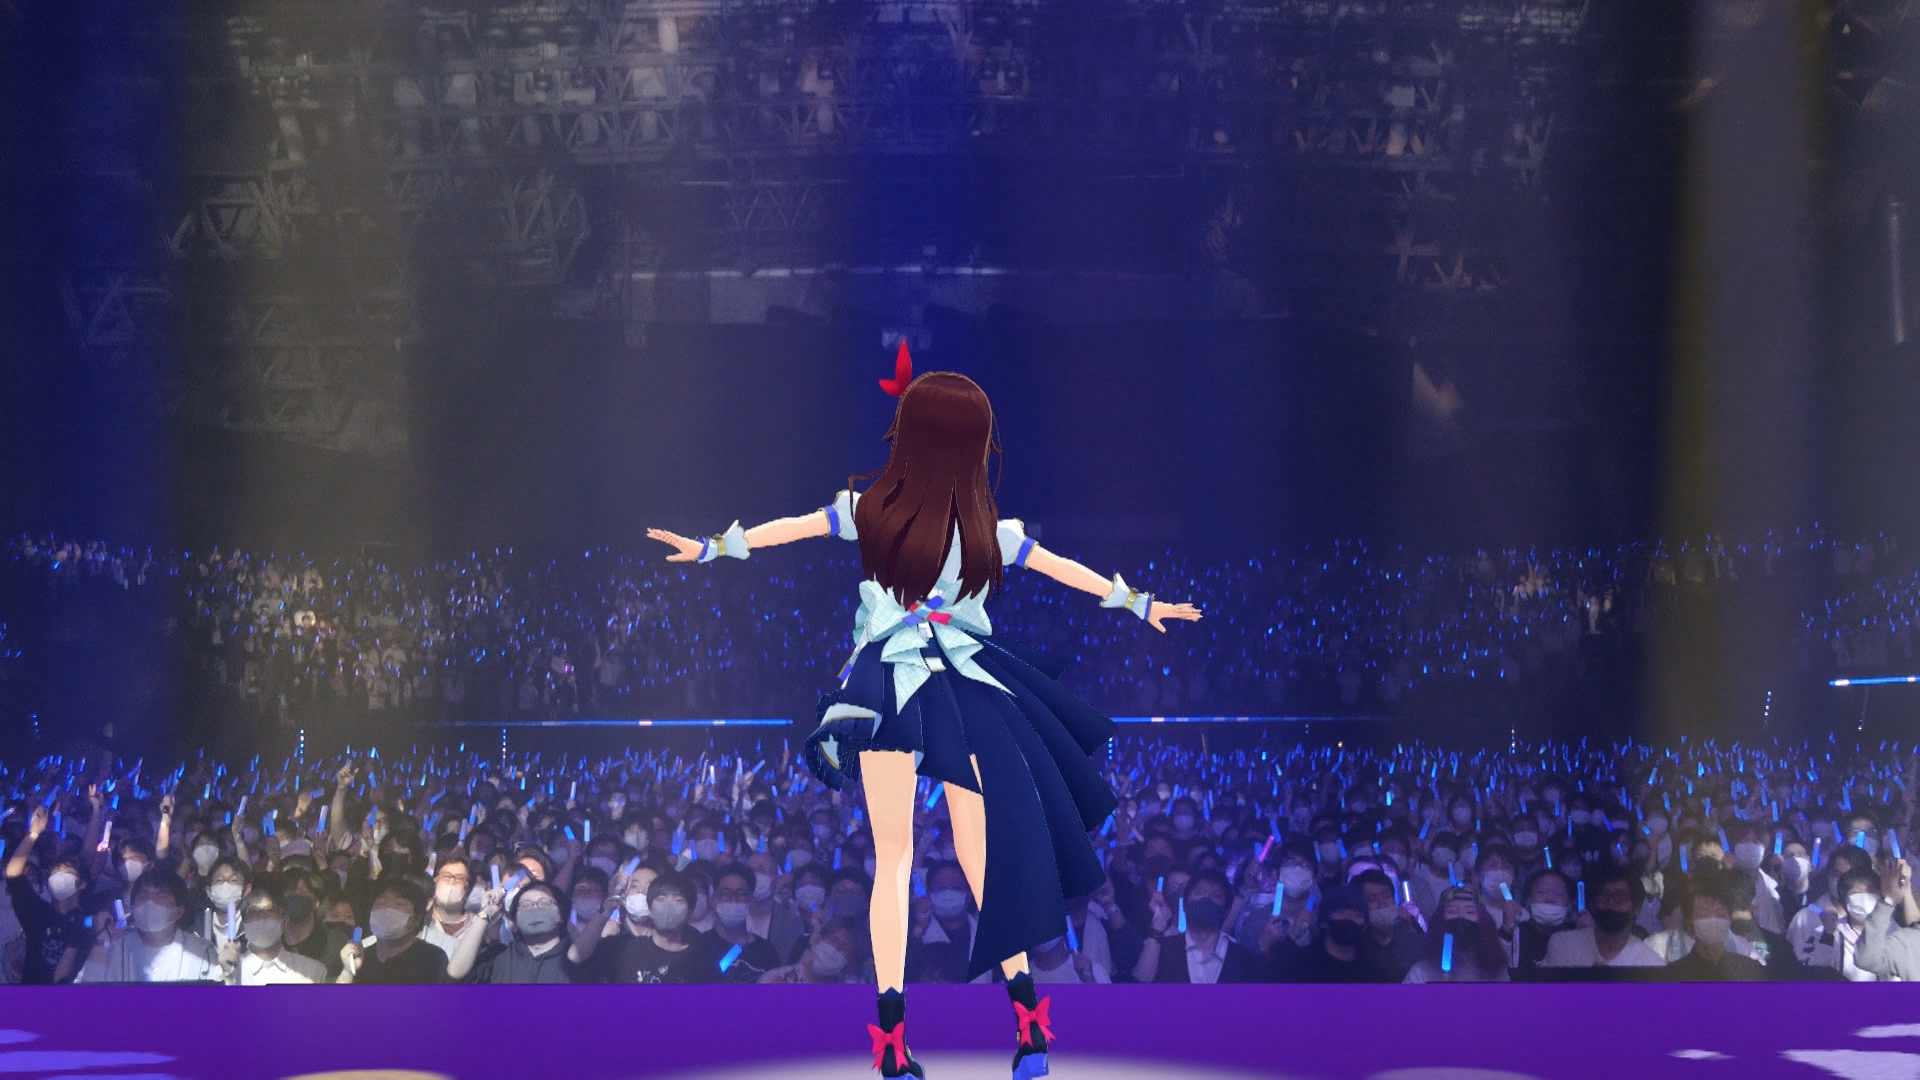
\includegraphics[width=.8\linewidth]{images/sora_performing.png}
    \vspace{0.2em}
    \parbox{\linewidth}{\centering \tiny Tokino Sora performs Yumezora$\bigstar$Fanfare \begin{CJK}{UTF8}{min}ユメゾラ$\bigstar$ファンファーレ\end{CJK} in front of the hololive 4th fes. crowd on March 18, 2023}
\end{frame}
\end{document}
